\documentclass{beamer}

\usepackage[utf8]{inputenc}
\usepackage[spanish]{babel}
\usepackage[T1]{fontenc}
\usepackage{graphicx}
\usepackage{tikz}
\usepackage{listings}

% \usepackage{pgfpages}
% \pgfpagesuselayout{2 on 1}[a4paper,border shrink=5mm]

\renewcommand\shorthandsspanish{}
\noextrasspanish

\title{Python como Entorno Científico de Desarrollo}
\author{
Guillem Borrell i Nogueras\\
\texttt{guillem@torroja.dmt.upm.es}\\
Segunda sesión
}

\begin{document}

\lstset{language=Python,
  backgroundcolor=\color{black!20},
  numbers=left,
  basicstyle=\small\ttfamily,
  keywordstyle=\color{blue},
  extendedchars=true,
  inputencoding=utf8,
  showspaces=false}

\begin{frame}
\begin{center}
 
\includegraphics[width=9cm]{files/python-logo-generic.pdf}\\
 % python-logo-generic.pdf: 389x115 pixel, 72dpi, 13.72x4.06 cm, bb=0 0 389 115
\begin{large}
\textbf{Python como Entorno de Desarrollo Científico}
\end{large}\\

Guillem Borrell i Nogueras\\

Curso i-MATH, Julio-Septiembre de 2008
\end{center}

\end{frame}

%%%%%%%%%%%%%% Objetos %%%%%%%%%%%%%%%%

\begin{frame}
  \frametitle{Orientación a objetos}
  \begin{itemize}
  \item Paradigma de implementación de algoritmos
  \item Pretende adaptarse a la realidad
  \item Estructura que puede contener datos y métodos
  \item Los objetos pueden relacionarse entre ellos mediante la
    herencia
  \item El método más común es generar una instancia a partir de una
    clase
  \end{itemize}
\end{frame}

\defverbatim[colored]\testcode{
\begin{lstlisting}
In [1]: import math as m

In [2]: class Complex(object):
   ...:     def __init__(self, realp, imagp):
   ...:         self.r = realp
   ...:         self.i = imagp
   ...:
   ...:     def abs(self):
   ...:         return m.sqrt(self.r**2+self.i**2)
   ...:
\end{lstlisting} 
}
\begin{frame}
  \frametitle{Orientación a objetos}
  \testcode
\end{frame}

\defverbatim[colored]\testcode{
\begin{lstlisting}
In [3]: nc = Complex(3,4)#instancia de clase

In [4]: nc.r
Out[4]: 3

In [5]: nc.i
Out[5]: 4

In [6]: nc.abs()
Out[6]: 5.0
\end{lstlisting} 
}
\begin{frame}
  \frametitle{Orientación a objetos}
  \testcode
\end{frame}

\begin{frame}
  \frametitle{Herencia}
  \begin{itemize}
  \item El mecanismo de extensión es la herencia
  \item Sirve para crear una \emph{jerarquía} de objetos
  \item Si una clase cede su contenido se llama clase \emph{padre} o
    \emph{parent}
  \item La clase que se genera a partir de la \emph{parent} es la
    clase \emph{hijo}
  \item Una clase puede heredar de varias clases superiores.
  \end{itemize}
\end{frame}


\defverbatim[colored]\testcode{
\begin{lstlisting}
class MoreComplex(Complex):
    def __init__(self, realp, imagp):
        Complex.__init__(self,realp,imagp)

    def arg(self):
        return m.atan(self.i/self.r)

In [14]: mc = MoreComplex(3,4)

In [15]: mc.arg()
Out[15]: 0.78539816339744828
\end{lstlisting} 
}
\begin{frame}
  \frametitle{Herencia}
  \testcode
\end{frame}


\defverbatim[colored]\testcode{
\begin{lstlisting}
 >>> class pato:
...     cantidad = 1
...     def haz_cua(self):
...           print "cua!"
...
...     def reproducete(self):
...           cantidad += 1
...
>>> estoesunpato=pato() #instancia de pato
>>> estoesunpato.cantidad
1
>>> estoesunpato.haz_cua()
cua!
\end{lstlisting} 
}

\begin{frame}
\frametitle{Duck typing}
\testcode
\end{frame}

\defverbatim[colored]\testcode{
\begin{lstlisting}
>>> estoesunpato=pato() #instancia de pato
>>> cuaqueador(estoesunpato)
cua!
>>> class guillem:
...     def haz_cua(self):
...             print "cua!"
...
>>> falsopato=guillem() #ese soy yo
>>> cuaqueador(falsopato)
cua!
>>> isinstance(falsopato,pato)
False
\end{lstlisting}
}
\begin{frame}
\frametitle{Duck typing}
\testcode

Si algo anda como un pato y hace cua como un pato para mi va a ser un pato.
Para la función cuaqueador yo soy tan pato como un pato.
\end{frame}

\begin{frame}
  \frametitle{Ejercicio}

\end{frame}

%%%%%%%%%%% NumPy y SciPy %%%%%%%%%%%%%

\begin{frame}
  \frametitle{Numpy}
  
\end{frame}

\begin{frame}
  \frametitle{Scipy}
  
\end{frame}


\begin{frame}
  \frametitle{Sage}
  
\end{frame}
%%%%%%%%%%%%%%%% HPC %%%%%%%%%%%%%%%%%%


\begin{frame}
 \frametitle{python para castañas (grandes)}
  \begin{center}
 \begin{tabular}[h]{ccc}
   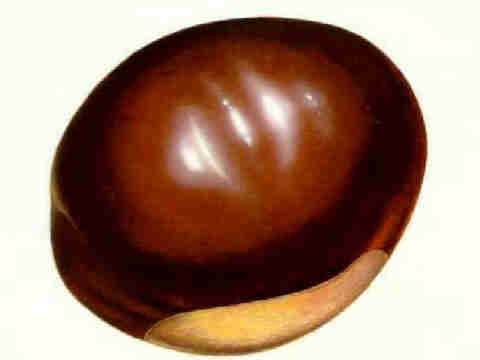
\includegraphics[width=5cm]{files/castana.jpg}& &
   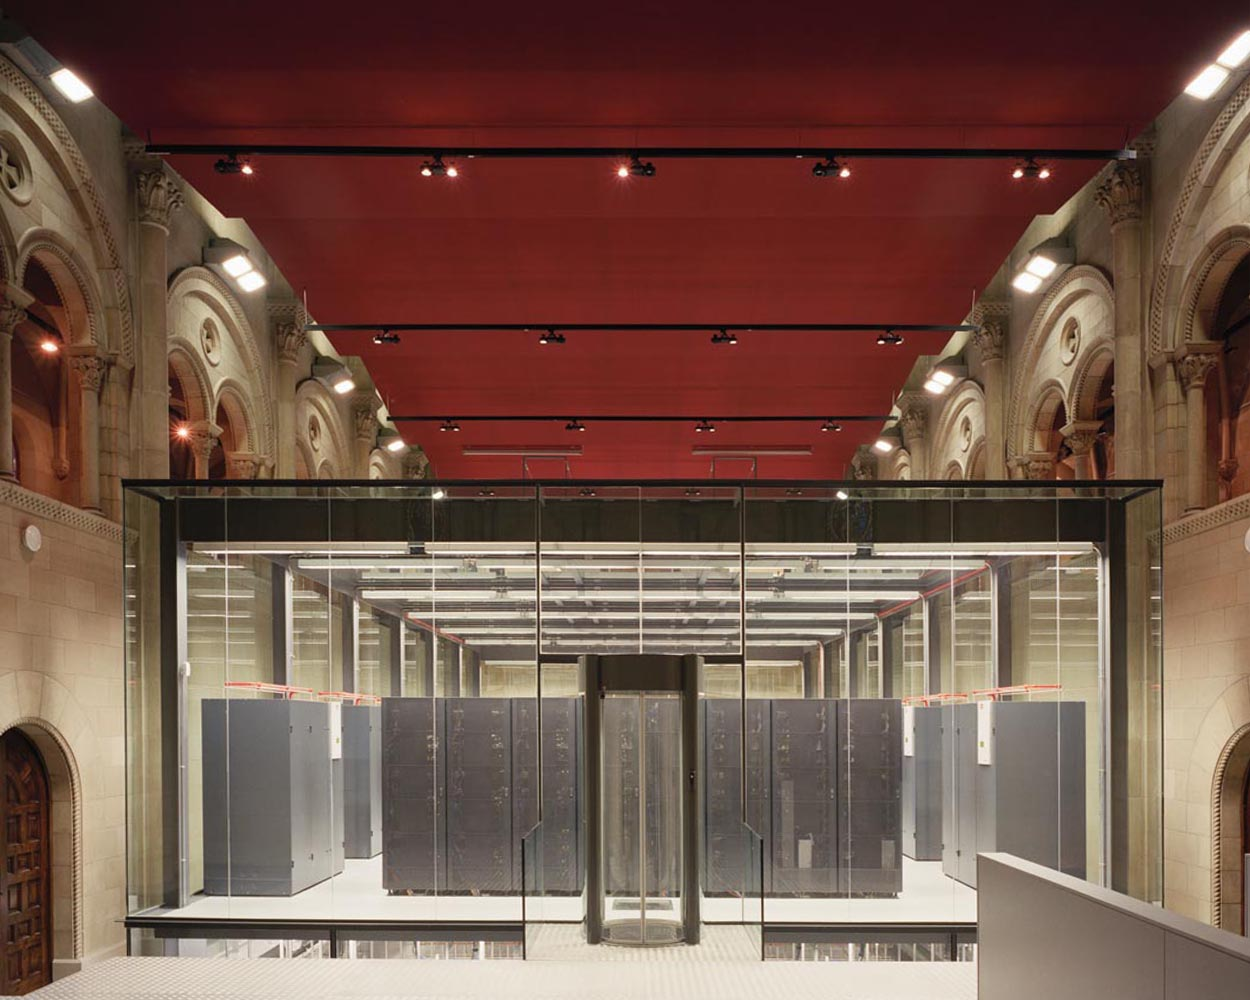
\includegraphics[width=5cm]{files/marenostrum.jpg}\\
   Castaña & = & Grande
 \end{tabular}
\end{center}
\end{frame}

\begin{frame}
  \frametitle{Same old story}
  \begin{center}
    \begin{Huge}
      \textbf{HPC = Fortran, C}
    \end{Huge}
  \end{center}
\end{frame}

\begin{frame}
  \frametitle{Ganaremos}
  \begin{itemize}
  \item Velocidad
  \item Gestión directa de la memoria
  \item ¿Algo más?
  \end{itemize}
\end{frame}

\begin{frame}
  \frametitle{Perderemos:}
  \begin{itemize}
  \item Interactividad
  \item Garbage collection
  \item Versatilidad
  \item Sencillez
  \item Librerías
  \end{itemize}
\end{frame}

\begin{frame}
  \begin{center}
    \begin{LARGE}
    ¿Podemos quedarnos con lo mejor de los dos mundos?      
    \end{LARGE}
  \end{center}
\end{frame}

\begin{frame}
  \frametitle{¿Por qué los lenguajes interpretados son lentos?}
  Porque son dinámicos.
  \begin{center}
    \begin{tikzpicture}      
      \node (lexer) at (0,0) [draw=black, thick, fill=black!10]
      {Lexer};

      \node (parser) at (2,0) [draw=black, thick, fill=black!10]
      {Parser};

      \node (encoder) at (4,0) [draw=black, thick, fill=black!10]
      {Encoder};

      \node (vm) at (7,0) [draw=black, very thick, fill=black!10]
      {VM};

      \node (codigo) at (0,1) [draw=blue,rounded
      corners,thick,fill=blue!20] {Codigo};

      \node (tokens) at (1,-1) [draw=blue,rounded
      corners,thick,fill=blue!20]
      {Tokens};

      \node (tokensp) at (3,1) [draw=blue,rounded
      corners,thick,fill=blue!20]
      {Tree};

      \node (bytecode) at (5.5,-1) [draw=blue,rounded
      corners,thick,fill=blue!20]
      {Bytecode};

      \node (assembler) at (8.5,1) [draw=blue,rounded
      corners,thick,fill=blue!20]
      {Assembler};
      
      \draw[->] (codigo.south) -- (lexer.north);

      \draw[->] (lexer.south) |- (tokens.west);

      \draw[->] (tokens.east) -| (parser.south);

      \draw[->] (parser.north) |- (tokensp.west);

      \draw[->] (tokensp.east) -| (encoder.north);

      \draw[->] (encoder.south) |- (bytecode.west);

      \draw[->] (bytecode.east) -| (vm.south);
      
      \draw[->] (vm.north) |- (assembler.west);
    \end{tikzpicture}
  \end{center}

\end{frame}

\begin{frame}
  \frametitle{Lenguajes dinámicos}
  \begin{itemize}
  \item El tipo de las variables sólo se sabe en tiempo de ejecución.
  \item El bytecode mueve un \textit{objectspace} o \textit{stack}
  \item El ensamblador de la máquina virtual hace lo que le dice el
    bytecode.
  \item La máquina virtual es incapaz de generar ensamblador
    optimizado.
  \item Dos planteamientos para lenguajes dinámicos
    \begin{itemize}
    \item Duck typing
    \item Type inference
    \end{itemize}
  \end{itemize}
\end{frame}

\begin{frame}
  \frametitle{Type inference}
  \begin{itemize}
  \item Intenta descubrir los tipos de cada variable en tiempo de
    compilación.
  \item El lenguaje es dinámico en apariencia pero estático en
    memoria.
  \item Menos dinámico que el Duck typing.
    \begin{itemize}
    \item Errores en tiempo de compilación
    \item Casting automático.
    \end{itemize}
  \item Mejor rendimiento.
  \end{itemize}
\end{frame}

\begin{frame}
  \frametitle{JIT}
  Just In Time
  \begin{itemize}
  \item Método para optimizar el bytecode.
    \begin{itemize}
    \item Analiza el bytecode.
    \item Hace type inference.
    \item Genera ensamblador optimizado para la arquitectura.
    \end{itemize}
  \item Matlab lo utiliza para los bucles.
  \item Octave va detrás de ello.
  \item Python no tiene... PyPy sí, aunque muy verde.
  \end{itemize}
\end{frame}

\begin{frame}
  \frametitle{Global Interpreter Lock}
  Otro problema de python (y otros).
  \begin{itemize}
  \item La máquina virtual sólo puede ejecutar un thread.
  \item No tendremos multithreading por muy trivial que quede en el
    bytecode.
  \item Si queremos threads tendremos que pedirlos
  \item Estensiones con propia gestión de threads.
  \item Con un poco de suerte se arreglará, de otra forma python
    morirá.
  \end{itemize}
\end{frame}

\begin{frame}
  \frametitle{La solución}
  \begin{center}
    \begin{Huge}
      Optimización Selectiva
    \end{Huge}
  \end{center}
  \vspace{1cm}
  \begin{flushright}
    \textit{We should forget about small efficiencies, say about 97\%
      of the time: premature optimization is the root of all evil. Yet
      we should not pass up our opportunities in that critical 3\%}. Knuth
  \end{flushright}
\end{frame}

\begin{frame}
  \frametitle{La regla del 80-20}
  \begin{itemize}
  \item El 80\% del código se escribe en el 20\% de tiempo.
  \item El 80\% del código es para tareas triviales, sólo el 20\%
    calcula algo de verdad.
  \item Del anterior, sólo el 20\% es realmente intensivo.
  \item Ergo sólo tendremos que optimizar un 5\% del código.
  \end{itemize}
\end{frame}

\begin{frame}
  \frametitle{Estrategia a seguir}
  \begin{flushright}
    \textit{Bottlenecks occur in surprising places, so don't try to
      second guess and put in a speed hack until yo have proven that's
      where the bottleneck is}. Rob Pike
  \end{flushright}
  \vspace{1cm}
  \begin{itemize}
  \item Hacer un buen profiling del código.
  \item Descubrir los cuellos de botella.
  \item \textbf{Eliminar el componente dinámico del lenguaje donde sea
    estrictamente necesario.}
  \end{itemize}
\end{frame}

\begin{frame}
  \begin{center}
    \begin{Huge}
      Siempre que no tengamos que paralelizar.
    \end{Huge}
  \end{center}
\end{frame}


\begin{frame}
  \frametitle{Para ello...}
  \begin{itemize}
  \item Escribir extensiones a la Máquina virtual con C (Python.h)
  \item Escribir módulos en Fortran (f2py)
  \item Enlazar al intérprete bibliotecas en C o Fortran (ctypes,
    swig)
  \item Utilizar un lenguaje de extensión (pyrex, cython)
  \item Crear nuestra propia versión de python (PyPy)
  \item[$\rightarrow$] Utilizar un intérprete preparado para el cálculo paralelo
    (ipython1)
  \end{itemize}
\end{frame}

\begin{frame}
\begin{center}
 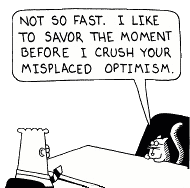
\includegraphics[width=6cm]{files/catbert.png}\\
\end{center}
\end{frame}

\beamertemplatesolidbackgroundcolor{red}

\begin{frame}
  \begin{center}
    \begin{Huge}
      \color{white}{\textbf{¿Con cuál me quedo?}}
    \end{Huge}
  \end{center}
\end{frame}

\beamertemplatesolidbackgroundcolor{white}

\begin{frame}
  \frametitle{Profiling}
\defverbatim[colored]\testcode{
\begin{lstlisting}
$ python -m profile main.py
         101006 function calls (96090 primitive calls) in 1.740 CPU seconds

   Ordered by: standard name

   ncalls  tottime  percall  cumtime  percall filename:lineno(function)
        1    0.000    0.000    0.000    0.000 :0(__import__)
        2    0.000    0.000    0.000    0.000 :0(__new__)
       15    0.000    0.000    0.000    0.000 :0(_getframe)
      589    0.000    0.000    0.000    0.000 :0(abs)
       38    0.000    0.000    0.000    0.000 :0(acquire_lock)
      144    0.000    0.000    0.000    0.000 :0(add_docstring)
        2    0.000    0.000    0.000    0.000 :0(allocate_lock)
\end{lstlisting}
}  
\end{frame}

\begin{frame}
  \frametitle{Pyrex}
  \begin{itemize}
  \item Lenguaje para escribir extensiones en python
  \item Menos dinámico que Python
  \item Un compilador lo traduce a C y genera el módulo que luego
    enlaza a CPython
  \item El proceso de creación del módulo es lento pero una vez se ha
    enlazado conseguimos velocidades parecidas a las de C.
  \end{itemize}
\end{frame}

\begin{frame}
  \frametitle{f2py}
  \begin{center}
    Una oportunidad de utilizar el lenguaje de programación del
    futuro, Fortran.
  \end{center}
\end{frame}

\begin{frame}
  \frametitle{PyPy}
  \begin{center}
    La revolución de la abstracción.
  \end{center}
\end{frame}
\end{document}
